\documentclass[12pt,a4paper]{article}

% ── Packages ──────────────────────────────────────────────────────────────────
\usepackage{amsmath,amssymb}
\usepackage[margin=2.5cm]{geometry}
\usepackage{booktabs}
\usepackage{xcolor}
\usepackage{hyperref}
\usepackage{listings}
\usepackage{pgfplots}
\pgfplotsset{compat=1.18}
\usepackage[most,breakable]{tcolorbox}
\tcbuselibrary{skins,breakable}
\usepackage{enumitem}
\usepackage{fancyhdr}
\usepackage{tikz}
\usepackage{array}

% ── tcolorbox environments ────────────────────────────────────────────────────
\newtcolorbox{curiositybox}[1]{colback=yellow!10, colframe=orange!80!black, fonttitle=\bfseries, title=#1, breakable}
\newtcolorbox{infobox}[1]{colback=blue!5, colframe=blue!60!black, fonttitle=\bfseries, title=#1, breakable}
\newtcolorbox{mistakebox}[1]{colback=red!5, colframe=red!60!black, fonttitle=\bfseries, title=#1, breakable}
\newtcolorbox{learnbox}[1]{colback=green!5, colframe=green!60!black, fonttitle=\bfseries, title=#1, breakable}

% ── lstlisting ────────────────────────────────────────────────────────────────
\lstset{language=Python, basicstyle=\ttfamily\small, keywordstyle=\color{blue},
        commentstyle=\color{gray}, stringstyle=\color{red},
        showstringspaces=false, breaklines=true, frame=single}

% ── fancyhdr ─────────────────────────────────────────────────────────────────
\pagestyle{fancy}
\fancyhf{}
\lhead{Topic 14: Zeros of Analytic Functions}
\rhead{Unit II --- Complex Variables}
\cfoot{\thepage}

% ── Title ─────────────────────────────────────────────────────────────────────
\title{\textbf{Topic 14: Zeros of Analytic Functions}\\[6pt]
       \large Unit II --- Complex Variable: Integration\\
       Complex Variables and Special Functions\\
       JNTUA College of Engineering (Autonomous)}
\author{B.Tech Engineering Students}
\date{}

% ══════════════════════════════════════════════════════════════════════════════
\begin{document}
\maketitle
\tableofcontents
\newpage

% ── Opening Hook ──────────────────────────────────────────────────────────────
\begin{curiositybox}{Hook}
A polynomial can have repeated roots like $(z-1)^3$. Analytic functions generalize this idea
in a beautiful way: zeros are not just points where the function becomes zero, they also carry
an \emph{order} or \emph{multiplicity}, and that order tells us a great deal about the local
behavior of the function. A simple zero behaves like a straight crossing; a double zero behaves
like a parabola touching the axis; a zero of order $m$ flattens the function against the axis
more and more dramatically as $m$ increases.
\end{curiositybox}

% ══════════════════════════════════════════════════════════════════════════════
\section{Definition of Zero}
% ══════════════════════════════════════════════════════════════════════════════

Before we study analytic functions in full generality, recall that for a real polynomial
$p(x) = a_0 + a_1 x + \cdots + a_n x^n$, a \emph{root} or \emph{zero} is any value $x_0$
with $p(x_0) = 0$. The same concept lifts cleanly to the complex plane.

\begin{infobox}{Definition --- Zero of an Analytic Function}
Let $f$ be analytic in a domain $D \subseteq \mathbb{C}$. A point $z_0 \in D$ is called a
\textbf{zero} of $f$ if
\[
  f(z_0) = 0.
\]
Equivalently, $z_0$ is a zero if and only if $z - z_0$ is a factor of $f$ in the sense that
$f(z) = (z-z_0)\,h(z)$ for some function $h$ analytic at $z_0$ (with $h$ possibly zero
at $z_0$ as well).
\end{infobox}

\subsection*{Polynomial Motivation}

Consider the following familiar examples in $\mathbb{C}$:

\begin{center}
\begin{tabular}{lll}
\toprule
\textbf{Function} & \textbf{Zeros} & \textbf{Observation}\\
\midrule
$f(z) = z^2 - 4$ & $z = 2,\; z = -2$ & Two distinct simple zeros\\
$f(z) = (z - 3)^2$ & $z = 3$ & One repeated zero\\
$f(z) = z^2 + 1$ & $z = i,\; z = -i$ & Zeros lie off the real axis\\
$f(z) = (z-1)(z+2i)^3$ & $z=1$ (simple), $z=-2i$ (order 3) & Mixed multiplicities\\
\bottomrule
\end{tabular}
\end{center}

Polynomials make zeros transparent, but the same structure persists for all analytic
functions via their Taylor series.

\begin{learnbox}{Key Takeaway --- Definition}
A zero of $f$ at $z_0$ means $f(z_0)=0$. Polynomial examples show that zeros can be simple
or repeated. For analytic functions the same classification is made precise through derivatives.
\end{learnbox}

% ══════════════════════════════════════════════════════════════════════════════
\section{Order / Multiplicity of a Zero}
% ══════════════════════════════════════════════════════════════════════════════

\begin{infobox}{Definition --- Order (Multiplicity) of a Zero}
Let $f$ be analytic at $z_0$ and let $f(z_0)=0$. The \textbf{order} (or \textbf{multiplicity})
of the zero at $z_0$ is the positive integer $m$ such that
\[
  f(z_0) = f'(z_0) = f''(z_0) = \cdots = f^{(m-1)}(z_0) = 0,
  \qquad \text{but} \qquad f^{(m)}(z_0) \neq 0.
\]
\begin{itemize}
  \item If $m=1$: the zero is called \textbf{simple}.
  \item If $m=2$: the zero is called a \textbf{double zero}.
  \item In general: a \textbf{zero of order $m$}.
\end{itemize}
\textbf{Derivative Test:} Compute successive derivatives of $f$ at $z_0$.
The order equals the index of the first non-vanishing derivative.
\end{infobox}

\subsection*{Geometric Interpretation}

Near a zero of order $m$, the function $f$ behaves like $c(z-z_0)^m$ for some constant
$c \neq 0$. This means:
\begin{itemize}
  \item $m=1$: $f$ crosses zero with non-zero slope --- a transversal crossing.
  \item $m=2$: $f$ touches zero and bounces back (like a parabola at its vertex).
  \item $m \geq 3$: $f$ is increasingly ``flat'' at $z_0$.
\end{itemize}

\begin{learnbox}{Key Takeaway --- Multiplicity}
The order $m$ of a zero is the smallest positive integer for which $f^{(m)}(z_0)\neq 0$.
Compute derivatives in order until one is non-zero; that index is the multiplicity.
\end{learnbox}

% ══════════════════════════════════════════════════════════════════════════════
\section{Taylor-Series Viewpoint}
% ══════════════════════════════════════════════════════════════════════════════

\begin{infobox}{Factored Form via Taylor Series}
If $f$ is analytic at $z_0$ and has a zero of order $m$ there, then the Taylor series
\[
  f(z) = \sum_{k=0}^{\infty} \frac{f^{(k)}(z_0)}{k!}(z-z_0)^k
\]
has $a_0 = a_1 = \cdots = a_{m-1} = 0$ and $a_m \neq 0$. Factoring out $(z-z_0)^m$:
\[
  \boxed{f(z) = (z-z_0)^m \, g(z)},
\]
where
\[
  g(z) = \sum_{k=0}^{\infty} a_{m+k}(z-z_0)^k = a_m + a_{m+1}(z-z_0) + \cdots
\]
is analytic at $z_0$ and satisfies $g(z_0) = a_m \neq 0$.
\end{infobox}

\subsection*{How the Factorization Arises}

Starting from the Taylor series of $f$ about $z_0$:
\[
  f(z) = a_m(z-z_0)^m + a_{m+1}(z-z_0)^{m+1} + a_{m+2}(z-z_0)^{m+2} + \cdots
\]
Factor out $(z-z_0)^m$:
\[
  f(z) = (z-z_0)^m \Bigl[a_m + a_{m+1}(z-z_0) + a_{m+2}(z-z_0)^2 + \cdots \Bigr]
       = (z-z_0)^m \, g(z).
\]
Since $g(z_0) = a_m \neq 0$ and the series for $g$ converges in a neighbourhood of $z_0$,
$g$ is analytic and non-zero near $z_0$.

\subsection*{Example}

Let $f(z) = \sin z$ near $z_0 = 0$. The Taylor series is
\[
  \sin z = z - \frac{z^3}{3!} + \frac{z^5}{5!} - \cdots = z\left(1 - \frac{z^2}{6} + \cdots\right).
\]
So $m=1$ and $g(z) = 1 - z^2/6 + \cdots$ with $g(0)=1 \neq 0$. The zero at $z_0=0$ is simple.

\begin{learnbox}{Key Takeaway --- Factored Form}
$f(z)=(z-z_0)^m g(z)$ with $g(z_0)\neq 0$ is the canonical way to encode a zero of order $m$.
The Taylor series makes the derivation mechanical: just identify the first non-zero coefficient.
\end{learnbox}

% ══════════════════════════════════════════════════════════════════════════════
\section{Isolated Nature of Zeros}
% ══════════════════════════════════════════════════════════════════════════════

\begin{infobox}{Theorem --- Zeros are Isolated}
If $f$ is analytic in a domain $D$ and $f$ is not identically zero, then the zeros of $f$
are \textbf{isolated}: for every zero $z_0$ there exists $r > 0$ such that the punctured
disc $0 < |z - z_0| < r$ contains no zeros of $f$.
\end{infobox}

\subsection*{Proof Sketch}

Since $f(z_0)=0$ with order $m$, we have $f(z)=(z-z_0)^m g(z)$ where $g(z_0)\neq 0$.
Because $g$ is continuous at $z_0$, there is a disc $|z-z_0|<r$ in which $g(z)\neq 0$.
In this disc, $f(z)=0$ only if $(z-z_0)^m=0$, i.e.\ only at $z=z_0$ itself. Hence no
other zeros exist within distance $r$ of $z_0$.

\subsection*{Consequence: Identity Theorem}

If two analytic functions $f$ and $g$ agree on a set that has a limit point in $D$,
then $f \equiv g$ throughout $D$. This follows because the zeros of $f-g$ would not
be isolated, forcing $f-g \equiv 0$.

\subsection*{Contrast with Real Analysis}

The real function $h(x) = x^2 \sin(1/x)$ (with $h(0)=0$) has zeros accumulating at
$x=0$, yet $h$ is not identically zero. Such behaviour is \emph{impossible} for a
non-trivial analytic function of a complex variable.

\begin{learnbox}{Key Takeaway --- Isolated Zeros}
Non-trivial analytic functions cannot have zeros that accumulate. Each zero sits in a
small punctured disc that is zero-free. This ``rigidity'' is one of the most powerful
features of complex analysis.
\end{learnbox}

% ══════════════════════════════════════════════════════════════════════════════
\section{Examples of Zeros in Standard Functions}
% ══════════════════════════════════════════════════════════════════════════════

\begin{infobox}{Standard Functions and Their Zeros}
\begin{center}
\begin{tabular}{>{\raggedright}p{4.2cm} >{\raggedright}p{4.2cm} >{\raggedright\arraybackslash}p{3.8cm}}
\toprule
\textbf{Function} & \textbf{Zeros} & \textbf{Order}\\
\midrule
$f(z)=z^3-8$ & $z=2,\;2e^{2\pi i/3},\;2e^{4\pi i/3}$ & Each simple ($m=1$)\\[4pt]
$f(z)=\sin z$ & $z = n\pi,\; n\in\mathbb{Z}$ & Each simple ($m=1$)\\[4pt]
$f(z)=(z-i)^3$ & $z=i$ & Order $m=3$\\[4pt]
$f(z)=1-\cos z$ & $z=2n\pi,\; n\in\mathbb{Z}$ & Order $m=2$\\[4pt]
$f(z)=z^2(z+1)$ & $z=0$ (order 2), $z=-1$ (simple) & Mixed\\[4pt]
$f(z)=e^z - 1$ & $z=2n\pi i,\; n\in\mathbb{Z}$ & Each simple\\
\bottomrule
\end{tabular}
\end{center}
\end{infobox}

\subsection*{Verification: $\sin z$ zeros are simple}

$\frac{d}{dz}\sin z = \cos z$. At $z = n\pi$: $\cos(n\pi) = (-1)^n \neq 0$. Hence all
zeros of $\sin z$ are simple.

\subsection*{Verification: $1-\cos z$ has order-2 zeros}

Let $f(z) = 1 - \cos z$.
\[
  f(2n\pi) = 1 - 1 = 0,\quad
  f'(z) = \sin z,\quad f'(2n\pi) = 0,\quad
  f''(z) = \cos z,\quad f''(2n\pi) = 1 \neq 0.
\]
So $m = 2$ at each $z = 2n\pi$.

\begin{learnbox}{Key Takeaway --- Standard Functions}
Always verify multiplicity by computing derivatives in sequence until you find the
first non-zero value. Standard functions like $\sin z$, $1-\cos z$, and $e^z-1$ appear
repeatedly in applications; knowing their zero orders by heart is essential.
\end{learnbox}

% ══════════════════════════════════════════════════════════════════════════════
\section{Worked Examples}
% ══════════════════════════════════════════════════════════════════════════════

% ── Example 1 ─────────────────────────────────────────────────────────────────
\subsection*{Example 1: Order of zero of $f(z) = z^3 - 3z^2 + 3z - 1$}

\textbf{Find the zeros and their orders.}

Factor: $z^3 - 3z^2 + 3z - 1 = (z-1)^3$. So $z_0 = 1$ is the only zero.

\medskip\noindent\textbf{Derivative test:}
\begin{align*}
  f(1)   &= (1-1)^3 = 0,\\
  f'(z)  &= 3(z-1)^2,\quad f'(1)=0,\\
  f''(z) &= 6(z-1),\quad f''(1)=0,\\
  f'''(z)&= 6,\quad f'''(1)=6\neq 0.
\end{align*}
Hence the zero at $z_0 = 1$ has order $m = 3$.

\begin{learnbox}{Key Result --- Example 1}
$f(z)=(z-1)^3$ has a single zero at $z=1$ of order 3. Three consecutive derivatives
vanish before the third derivative gives $6\neq 0$.
\end{learnbox}

% ── Example 2 ─────────────────────────────────────────────────────────────────
\subsection*{Example 2: Zeros of $f(z) = z^2 + 4$}

\textbf{Find and classify the zeros.}

Set $f(z)=0$: $z^2 = -4 \Rightarrow z = \pm 2i$.

\medskip\noindent\textbf{Check each zero:}

For $z_0 = 2i$: $f'(z)=2z$, so $f'(2i)=4i\neq 0$. Hence $m=1$ (simple).

For $z_0 = -2i$: $f'(-2i)=-4i\neq 0$. Hence $m=1$ (simple).

Both zeros are simple.

\begin{learnbox}{Key Result --- Example 2}
$z^2+4$ has two simple zeros at $z=2i$ and $z=-2i$. Since the derivative is non-zero at
each, no further checking is needed.
\end{learnbox}

% ── Example 3 ─────────────────────────────────────────────────────────────────
\subsection*{Example 3: Order of zero of $f(z) = \sin^2 z$ at $z = 0$}

$f(z) = \sin^2 z$. Near $z=0$: $\sin z = z - z^3/6 + \cdots$, so
$\sin^2 z = z^2\!\left(1 - z^2/6 + \cdots\right)^{\!2} = z^2\!\left(1 - z^2/3 + \cdots\right)$.

The first non-zero term is $z^2$, so $m = 2$.

\medskip\noindent\textbf{Derivative verification:}
\begin{align*}
  f(z)   &= \sin^2 z,\quad f(0)=0,\\
  f'(z)  &= 2\sin z\cos z = \sin 2z,\quad f'(0)=0,\\
  f''(z) &= 2\cos 2z,\quad f''(0) = 2 \neq 0.
\end{align*}
So $m=2$ confirmed.

\begin{learnbox}{Key Result --- Example 3}
Squaring a function of order $m$ gives a function of order $2m$. Here $\sin z$ has a
simple zero at 0, so $\sin^2 z$ has a zero of order 2.
\end{learnbox}

% ── Example 4 ─────────────────────────────────────────────────────────────────
\subsection*{Example 4: Zeros of $f(z) = (z-2i)^3 (z+3)^2$}

The zeros are $z_0 = 2i$ (order 3) and $z_0 = -3$ (order 2).

\medskip\noindent\textbf{Derivative verification for $z_0=-3$:}
\begin{align*}
  f(z)   &= (z-2i)^3(z+3)^2,\quad f(-3)=(-3-2i)^3\cdot 0 = 0.\\
  f'(z)  &= 3(z-2i)^2(z+3)^2 + 2(z-2i)^3(z+3),\\
  f'(-3) &= 3(-3-2i)^2\cdot 0 + 2(-3-2i)^3\cdot 0 = 0.\\
  f''(z) &= 6(z-2i)(z+3)^2 + \text{terms with }(z+3),\\
  f''(-3)&= 6(-3-2i)(0)^2 + [\text{terms still contain }(z+3)\text{ or }(z+3)^2\text{ at }-3]\cdots
\end{align*}
More cleanly: write $f(z)=(z+3)^2 h(z)$ where $h(z)=(z-2i)^3$.
Then $h(-3)=(-3-2i)^3 \neq 0$, so by definition $z=-3$ has order 2.

\begin{learnbox}{Key Result --- Example 4}
When $f$ is given in factored form $(z-z_0)^m h(z)$ with $h(z_0)\neq 0$, the order is
immediately $m$. No derivative computation is needed; just read off the exponent.
\end{learnbox}

% ── Example 5 ─────────────────────────────────────────────────────────────────
\subsection*{Example 5: Order of zero of $f(z) = 1 - e^z$ at $z = 2\pi i$}

We need to test whether $f(2\pi i)=0$:
$e^{2\pi i} = \cos 2\pi + i\sin 2\pi = 1$, so $f(2\pi i)=1-1=0$. \checkmark

\medskip
$f'(z) = -e^z$, so $f'(2\pi i)=-e^{2\pi i}=-1\neq 0$.

Hence the zero is \textbf{simple} ($m=1$).

\begin{learnbox}{Key Result --- Example 5}
$1-e^z$ has infinitely many zeros at $z=2n\pi i$, $n\in\mathbb{Z}$, each of order 1.
The derivative $-e^z$ is never zero, so none of these zeros is repeated.
\end{learnbox}

% ── Example 6 ─────────────────────────────────────────────────────────────────
\subsection*{Example 6: Order of zero of $f(z) = z - \sin z$ at $z = 0$}

$f(0)=0-0=0$. Expand $\sin z$:
\[
  \sin z = z - \frac{z^3}{6} + \frac{z^5}{120} - \cdots
  \implies z - \sin z = \frac{z^3}{6} - \frac{z^5}{120} + \cdots = z^3\!\left(\frac{1}{6} - \frac{z^2}{120}+\cdots\right).
\]
So $m=3$ and $g(z)= \tfrac{1}{6} - \tfrac{z^2}{120}+\cdots$ with $g(0)=\tfrac{1}{6}\neq 0$.

\medskip\noindent\textbf{Derivative verification:}
\begin{align*}
  f'(z)   &= 1 - \cos z,\quad f'(0)=0.\\
  f''(z)  &= \sin z,\quad f''(0)=0.\\
  f'''(z) &= \cos z,\quad f'''(0)=1\neq 0.
\end{align*}
Confirmed: $m=3$.

\begin{learnbox}{Key Result --- Example 6}
$z-\sin z$ vanishes at $z=0$ to order 3. The Taylor series approach gives the answer
immediately; derivatives confirm it.
\end{learnbox}

% ── Example 7 ─────────────────────────────────────────────────────────────────
\subsection*{Example 7: Find the order of zero of $f(z)=\cos z - 1 + \tfrac{z^2}{2}$ at $z=0$}

Taylor expand $\cos z$:
\[
  \cos z = 1 - \frac{z^2}{2} + \frac{z^4}{24} - \cdots
  \implies \cos z - 1 + \frac{z^2}{2} = \frac{z^4}{24} - \frac{z^6}{720} + \cdots = z^4\!\left(\frac{1}{24} - \frac{z^2}{720}+\cdots\right).
\]
So $m=4$ and $g(0)=1/24\neq 0$.

\medskip\noindent\textbf{Derivative verification:}
\begin{align*}
  f(z) &= \cos z - 1 + \tfrac{z^2}{2},\quad f(0)=0.\\
  f'(z) &= -\sin z + z,\quad f'(0)=0.\\
  f''(z) &= -\cos z + 1,\quad f''(0)=0.\\
  f'''(z) &= \sin z,\quad f'''(0)=0.\\
  f^{(4)}(z) &= \cos z,\quad f^{(4)}(0)=1\neq 0.
\end{align*}
Confirmed: $m=4$.

\begin{learnbox}{Key Result --- Example 7}
Subtracting leading Taylor terms of $\cos z$ cancels the first three zero coefficients,
leaving a zero of order 4. Always use Taylor series when derivatives become tedious.
\end{learnbox}

% ── TikZ Diagram ──────────────────────────────────────────────────────────────
\subsection*{Visual: Behaviour Near Zeros of Different Orders}

\begin{center}
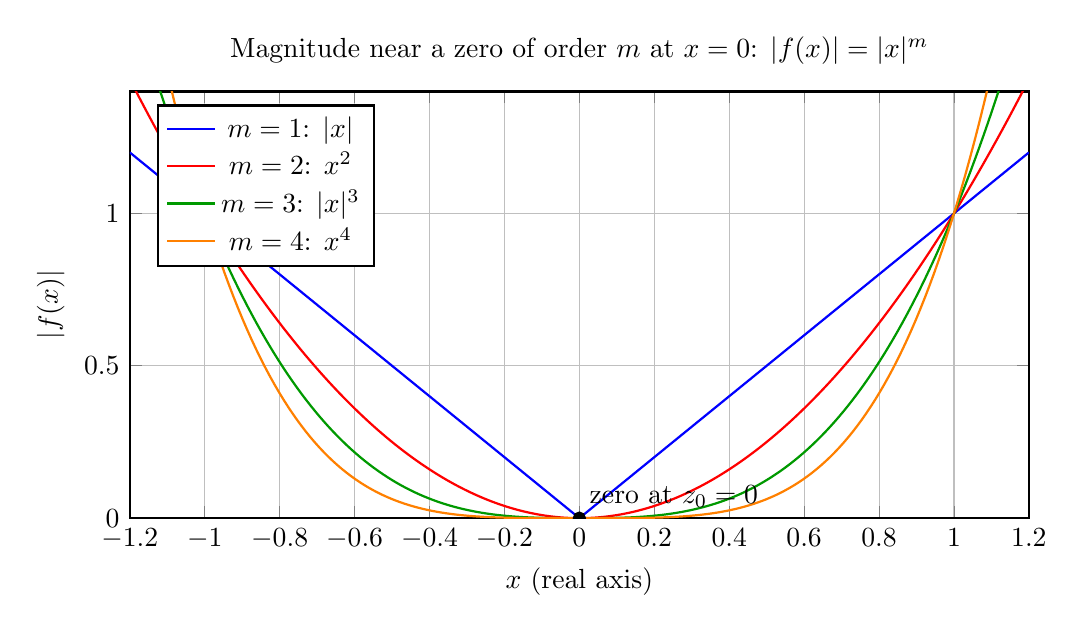
\begin{tikzpicture}
  \begin{axis}[
    width=13cm, height=7cm,
    xlabel={$x$ (real axis)},
    ylabel={$|f(x)|$},
    title={Magnitude near a zero of order $m$ at $x=0$: $|f(x)| = |x|^m$},
    xmin=-1.2, xmax=1.2, ymin=0, ymax=1.4,
    legend pos=north west,
    grid=major,
    thick
  ]
    \addplot[blue, domain=-1.2:1.2, samples=200]{abs(x)};
    \addlegendentry{$m=1$: $|x|$}
    \addplot[red, domain=-1.2:1.2, samples=200]{x*x};
    \addlegendentry{$m=2$: $x^2$}
    \addplot[green!60!black, domain=-1.2:1.2, samples=200]{abs(x)^3};
    \addlegendentry{$m=3$: $|x|^3$}
    \addplot[orange, domain=-1.2:1.2, samples=200]{x^4};
    \addlegendentry{$m=4$: $x^4$}
    \filldraw[black] (axis cs:0,0) circle (2pt) node[above right]{zero at $z_0=0$};
  \end{axis}
\end{tikzpicture}
\end{center}

Higher-order zeros produce a flatter ``touch'' at the zero; the function approaches zero
more gradually as $m$ increases.

% ══════════════════════════════════════════════════════════════════════════════
\section{Multiplicity Test Table (MANDATORY UPGRADE)}
% ══════════════════════════════════════════════════════════════════════════════

The table below summarises the complete derivative-based test for determining the order of
a zero $z_0$ of an analytic function $f$.

\begin{center}
\begin{tabular}{>{\raggedright}p{7.5cm} >{\raggedright\arraybackslash}p{6.5cm}}
\toprule
\textbf{Derivative Condition at $z = z_0$} & \textbf{Multiplicity Conclusion}\\
\midrule
$f(z_0)\neq 0$ & $z_0$ is \emph{not} a zero\\[4pt]
$f(z_0)=0$, $f'(z_0)\neq 0$ & Simple zero ($m=1$)\\[4pt]
$f(z_0)=f'(z_0)=0$, $f''(z_0)\neq 0$ & Double zero ($m=2$)\\[4pt]
$f(z_0)=f'(z_0)=f''(z_0)=0$, $f'''(z_0)\neq 0$ & Zero of order 3 ($m=3$)\\[4pt]
$f^{(k)}(z_0)=0$ for $k=0,1,\ldots,m-1$ and $f^{(m)}(z_0)\neq 0$ & Zero of order $m$\\[4pt]
$f^{(k)}(z_0)=0$ for all $k\geq 0$ & $f\equiv 0$ in $D$ (trivial function)\\
\bottomrule
\end{tabular}
\end{center}

\medskip

\begin{center}
\begin{tabular}{>{\raggedright}p{4.5cm} >{\raggedright}p{4.0cm} >{\raggedright\arraybackslash}p{5.0cm}}
\toprule
\textbf{Function} & \textbf{Zero at} & \textbf{Order (by test)}\\
\midrule
$z^4$ & $z=0$ & 4\\
$\sin z$ & $z=0$ & 1\\
$1-\cos z$ & $z=0$ & 2\\
$z - \sin z$ & $z=0$ & 3\\
$\cos z - 1 + z^2/2$ & $z=0$ & 4\\
$(z-1)^2(z+2)$ & $z=1$ & 2, $z=-2$: 1\\
$e^z - 1$ & $z=0$ & 1\\
$\sin^2 z$ & $z=0$ & 2\\
\bottomrule
\end{tabular}
\end{center}

\begin{learnbox}{Key Takeaway --- Multiplicity Table}
The derivative test is the universal procedure: evaluate $f$, $f'$, $f''$, \ldots at
$z_0$ in sequence. Stop at the first non-zero value; its index is $m$. If $f$ is given
in factored form $(z-z_0)^m g(z)$ with $g(z_0)\neq 0$, read off $m$ directly.
\end{learnbox}

% ══════════════════════════════════════════════════════════════════════════════
\section{Excel Example (MANDATORY)}
% ══════════════════════════════════════════════════════════════════════════════

\subsection*{Goal}

Numerically observe that a higher-order zero produces a flatter magnitude plot near $z_0$.
We evaluate $|f(x)| = |x|^m$ for $m = 1, 2, 3$ on the real axis near $x = 0$.

\subsection*{Spreadsheet Setup}

\begin{center}
\begin{tabular}{ccccc}
\toprule
\textbf{A} & \textbf{B} & \textbf{C} & \textbf{D} & \textbf{E}\\
\texttt{x} & \texttt{|x|\^{}1} & \texttt{|x|\^{}2} & \texttt{|x|\^{}3} & \texttt{Observation}\\
\midrule
$-0.50$ & \texttt{=ABS(A2)\^{}1} & \texttt{=ABS(A2)\^{}2} & \texttt{=ABS(A2)\^{}3} & Largest values away from 0\\
$-0.25$ & \texttt{=ABS(A3)\^{}1} & \texttt{=ABS(A3)\^{}2} & \texttt{=ABS(A3)\^{}3} & Values shrink toward 0\\
$-0.10$ & \texttt{=ABS(A4)\^{}1} & \texttt{=ABS(A4)\^{}2} & \texttt{=ABS(A4)\^{}3} & Higher order falls faster\\
$0.00$  & \texttt{=ABS(A5)\^{}1} & \texttt{=ABS(A5)\^{}2} & \texttt{=ABS(A5)\^{}3} & All zero at the zero\\
$0.10$  & \texttt{=ABS(A6)\^{}1} & \texttt{=ABS(A6)\^{}2} & \texttt{=ABS(A6)\^{}3} & Symmetric\\
$0.25$  & \texttt{=ABS(A7)\^{}1} & \texttt{=ABS(A7)\^{}2} & \texttt{=ABS(A7)\^{}3} & \\
$0.50$  & \texttt{=ABS(A8)\^{}1} & \texttt{=ABS(A8)\^{}2} & \texttt{=ABS(A8)\^{}3} & \\
\bottomrule
\end{tabular}
\end{center}

\subsection*{Computed Values}

\begin{center}
\begin{tabular}{ccccc}
\toprule
$x$ & $|x|^1$ & $|x|^2$ & $|x|^3$ & Observation\\
\midrule
$-0.50$ & 0.5000 & 0.2500 & 0.1250 & Largest; $m=1$ dominates\\
$-0.25$ & 0.2500 & 0.0625 & 0.0156 & Higher-order decays faster\\
$-0.10$ & 0.1000 & 0.0100 & 0.0010 & Dramatic difference\\
$0.00$  & 0.0000 & 0.0000 & 0.0000 & All models agree at zero\\
$0.10$  & 0.1000 & 0.0100 & 0.0010 & Symmetric\\
$0.25$  & 0.2500 & 0.0625 & 0.0156 & \\
$0.50$  & 0.5000 & 0.2500 & 0.1250 & \\
\bottomrule
\end{tabular}
\end{center}

\subsection*{Excel Chart Instructions}

\begin{enumerate}
  \item Select columns A through D.
  \item Insert $\to$ Line Chart.
  \item Label series: ``Order 1'', ``Order 2'', ``Order 3''.
  \item Add chart title: \textit{Magnitude near zero of order $m$}.
  \item Observe that for $|x|<0.25$, the order-3 curve lies far below the order-1 curve,
        confirming the flatter approach for higher multiplicity.
\end{enumerate}

\begin{learnbox}{Key Takeaway --- Excel}
Numerics confirm the theory: higher-order zeros produce smaller function values near $z_0$,
and the difference is dramatic for $|x| \ll 1$. This makes detection harder numerically
but the theory of derivatives resolves it exactly.
\end{learnbox}

% ══════════════════════════════════════════════════════════════════════════════
\section{Python Example (MANDATORY)}
% ══════════════════════════════════════════════════════════════════════════════

The following script uses \texttt{sympy} for symbolic computation to detect zeros and
determine their orders for several standard functions. It also uses \texttt{numpy} and
\texttt{matplotlib} to visualise the magnitude near a zero.

\begin{lstlisting}[language=Python]
import sympy as sp
import numpy as np
import matplotlib.pyplot as plt

z = sp.Symbol('z')

def zero_order(f_expr, z0, max_order=10):
    """Return the order of the zero of f at z0, or None if not a zero."""
    for m in range(max_order + 1):
        val = sp.diff(f_expr, z, m).subs(z, z0)
        val = sp.simplify(val)
        if val != 0:
            return m if m > 0 else None  # m=0 means f(z0) != 0
    return None  # all derivatives zero up to max_order

functions = [
    (z**3 - 3*z**2 + 3*z - 1, 1),   # (z-1)^3 at z=1
    (sp.sin(z),                 0),   # sin(z) at z=0
    (1 - sp.cos(z),             0),   # 1-cos(z) at z=0
    (z - sp.sin(z),             0),   # z-sin(z) at z=0
    (sp.cos(z) - 1 + z**2/2,   0),   # cos(z)-1+z^2/2 at z=0
    (sp.exp(z) - 1,             0),   # e^z-1 at z=0
]

print("=" * 52)
print(f"{'Function':<28} {'z0':>4} {'Order':>6}")
print("=" * 52)
for expr, z0 in functions:
    order = zero_order(expr, z0)
    name = str(expr)[:27]
    print(f"{name:<28} {z0:>4} {order:>6}")
print("=" * 52)

# Expected output:
# ====================================================
# Function                       z0  Order
# ====================================================
# z**3 - 3*z**2 + 3*z - 1        1      3
# sin(z)                          0      1
# 1 - cos(z)                      0      2
# z - sin(z)                      0      3
# cos(z) - 1 + z**2/2             0      4
# exp(z) - 1                      0      1
# ====================================================

# ── Visualisation: |x|^m near x=0 ─────────────────
x = np.linspace(-0.6, 0.6, 400)
fig, ax = plt.subplots(figsize=(8, 4))
for m, colour in zip([1, 2, 3, 4], ['blue', 'red', 'green', 'orange']):
    ax.plot(x, np.abs(x)**m, label=f'm={m}', color=colour)
ax.set_xlabel('x (real axis near zero)')
ax.set_ylabel('|f(x)| = |x|^m')
ax.set_title('Magnitude near a zero of order m at x=0')
ax.legend()
ax.grid(True)
plt.tight_layout()
plt.savefig('zeros_magnitude.png', dpi=150)
plt.show()
print("Plot saved to zeros_magnitude.png")
\end{lstlisting}

\begin{learnbox}{Key Takeaway --- Python}
\texttt{sympy.diff} combined with a loop over derivative orders provides an exact,
automatic multiplicity detector. The plot confirms the visual intuition: higher-order
zeros flatten the magnitude curve dramatically near $z_0$.
\end{learnbox}

% ══════════════════════════════════════════════════════════════════════════════
\section{Viva Questions (8)}
% ══════════════════════════════════════════════════════════════════════════════

\begin{enumerate}[label=\textbf{Q\arabic*.}]

\item \textbf{Define a zero of an analytic function.}\\
A point $z_0$ in the domain of an analytic function $f$ is called a zero if $f(z_0)=0$.

\item \textbf{What is the order (multiplicity) of a zero, and how is it determined?}\\
The order $m$ of a zero at $z_0$ is the smallest positive integer such that $f^{(m)}(z_0)\neq 0$
while $f(z_0)=f'(z_0)=\cdots=f^{(m-1)}(z_0)=0$. It is determined by computing successive
derivatives at $z_0$ until the first non-vanishing one is found.

\item \textbf{State the factored form of $f$ near a zero of order $m$.}\\
If $f$ has a zero of order $m$ at $z_0$, then $f(z)=(z-z_0)^m g(z)$ where $g$ is analytic
at $z_0$ and $g(z_0)\neq 0$.

\item \textbf{Why are zeros of a non-trivial analytic function isolated?}\\
Near $z_0$, $f(z)=(z-z_0)^m g(z)$ with $g(z_0)\neq 0$. By continuity, $g(z)\neq 0$ in some
disc $|z-z_0|<r$. In this disc $f(z)=0$ only at $z=z_0$ itself, so no zeros accumulate at $z_0$.

\item \textbf{What is a simple zero? Give an example.}\\
A simple zero is a zero of order 1, i.e.\ $f(z_0)=0$ but $f'(z_0)\neq 0$. Example: $f(z)=\sin z$
has a simple zero at $z=0$ because $\sin(0)=0$ and $\cos(0)=1\neq 0$.

\item \textbf{What is the order of the zero of $\sin z$ at $z=\pi$?}\\
$\sin(\pi)=0$ and $\frac{d}{dz}\sin z\big|_{z=\pi}=\cos(\pi)=-1\neq 0$. So the zero is simple ($m=1$).

\item \textbf{How does the Taylor series help identify the order of a zero?}\\
Expand $f$ in a Taylor series about $z_0$. The order $m$ equals the index of the first
non-zero coefficient $a_m$, since $f(z)=a_m(z-z_0)^m+\cdots$ with $a_m\neq 0$.

\item \textbf{Can a non-trivial analytic function have infinitely many zeros in a bounded closed
region?}\\
No. If $f$ is analytic and not identically zero in a domain, its zeros are isolated, so in
any bounded closed region the zeros form a finite set (a closed discrete set in a compact
space must be finite).

\end{enumerate}

% ══════════════════════════════════════════════════════════════════════════════
\section{Descriptive Questions (5)}
% ══════════════════════════════════════════════════════════════════════════════

\begin{enumerate}[label=\textbf{D\arabic*.}]

\item \textbf{State and prove that zeros of a non-constant analytic function are isolated.}\\
\textit{[Proof outline: Use $f(z)=(z-z_0)^m g(z)$ with $g(z_0)\neq 0$; invoke continuity of
$g$ to find a zero-free punctured disc.]}

\item \textbf{Derive the factored form $f(z)=(z-z_0)^m g(z)$ from the Taylor series of $f$ about
$z_0$, stating clearly the conditions on $g$.}\\
\textit{[Show that if $a_0=\cdots=a_{m-1}=0$ and $a_m\neq 0$, factoring out $(z-z_0)^m$ gives
$g(z)=\sum_{k\geq 0}a_{m+k}(z-z_0)^k$ analytic with $g(z_0)=a_m\neq 0$.]}

\item \textbf{Determine the order of the zeros of $f(z)=z^4 - 2z^3 + z^2$ at each of its zeros.
Show all derivative computations.}\\
\textit{[Factor: $z^2(z-1)^2$. Zero at $z=0$: order 2. Zero at $z=1$: order 2. Verify with
derivatives.]}

\item \textbf{Using the derivative test, find all zeros and their orders for
$f(z) = z^3\sin z$.}\\
\textit{[$z=0$: order 4 (from $z^3$ contributing 3 and $\sin z$ contributing 1);
$z=n\pi$ ($n\neq 0$): each is a simple zero.]}

\item \textbf{State the Identity Theorem for analytic functions and explain how it follows from
the isolated nature of zeros.}\\
\textit{[If $f$ and $g$ agree on a set with a limit point in domain $D$, then $f-g$ has
non-isolated zeros, forcing $f-g\equiv 0$ in $D$.]}

\end{enumerate}

% ══════════════════════════════════════════════════════════════════════════════
\section{Practice Problems (6)}
% ══════════════════════════════════════════════════════════════════════════════

\begin{enumerate}[label=\textbf{P\arabic*.}]

\item Find all zeros and their orders of $f(z)=z^5 - z^3$.\\
\textit{Hint: Factor $z^3(z^2-1)=z^3(z-1)(z+1)$. Zero at $z=0$ has order 3; zeros at $z=\pm 1$
are simple.}

\item Determine the order of the zero of $f(z)=\tan z - z$ at $z=0$.\\
\textit{Hint: Expand $\tan z = z + z^3/3 + \cdots$, so $\tan z - z = z^3/3 + \cdots$. Order is 3.}

\item Find the order of the zero of $f(z)=e^{z^2}-1$ at $z=0$.\\
\textit{Hint: $e^{z^2}-1 = z^2 + z^4/2 + \cdots = z^2(1+z^2/2+\cdots)$. Order is 2.}

\item Determine whether $z_0=i$ is a zero of $f(z)=(z^2+1)^3$ and find its order.\\
\textit{Hint: $(z^2+1)=(z-i)(z+i)$, so $(z^2+1)^3=(z-i)^3(z+i)^3$. At $z=i$: order 3.}

\item Show that all zeros of $f(z)=\cos z$ are simple.\\
\textit{Hint: Zeros at $z=(2n+1)\pi/2$; derivative $-\sin z$ at these points is
$\pm 1 \neq 0$.}

\item Find the zeros and their orders for $f(z)=(1-\cos z)\sin z$.\\
\textit{Hint: $1-\cos z$ has order-2 zeros at $z=2n\pi$; $\sin z$ has simple zeros at
$z=k\pi$. At $z=0$: orders add to give order 3; at $z=2n\pi$ ($n\neq 0$): order 2
from $1-\cos z$ and simple from $\sin z$ (if $2n\pi=k\pi$ then $\sin(2n\pi)=0$ too),
giving order 3; at $z=(2k+1)\pi$: simple zero from $\sin z$.}

\end{enumerate}

% ══════════════════════════════════════════════════════════════════════════════
\section{MCQs (5)}
% ══════════════════════════════════════════════════════════════════════════════

\begin{enumerate}[label=\textbf{MCQ\arabic*.}]

\item The order of the zero of $f(z) = (z-2)^4(z+1)$ at $z=2$ is:
\begin{enumerate}[label=(\alph*)]
  \item 1
  \item \textbf{4}
  \item 5
  \item 2
\end{enumerate}
\textit{Explanation: The factor $(z-2)^4$ contributes a zero of order 4 at $z=2$;
the factor $(z+1)$ is non-zero there.}

\item Which of the following is a zero of order 2 for $f(z)=\sin^2 z$?
\begin{enumerate}[label=(\alph*)]
  \item $z=\pi/2$
  \item \textbf{$z=0$}
  \item $z=\pi/4$
  \item $z=2\pi$
\end{enumerate}
\textit{Explanation: $\sin^2 z = z^2(1-z^2/3+\cdots)$, so the zero at $z=0$ has order 2.
$\sin(\pi/2)\neq 0$, $\sin(\pi/4)\neq 0$, $\sin(2\pi)=0$ but $\sin^2(2\pi)$ has order 2 there.}

\item The zeros of a non-trivial analytic function are:
\begin{enumerate}[label=(\alph*)]
  \item Dense in the domain
  \item Uncountable
  \item \textbf{Isolated}
  \item Always simple
\end{enumerate}
\textit{Explanation: By the factored form theorem, each zero lies in a punctured disc free
of other zeros, hence zeros are isolated.}

\item The order of the zero of $f(z)=z-\sin z$ at $z=0$ is:
\begin{enumerate}[label=(\alph*)]
  \item 1
  \item 2
  \item \textbf{3}
  \item 4
\end{enumerate}
\textit{Explanation: $z-\sin z = z^3/6 - z^5/120 + \cdots$, so the first non-zero term is $z^3$,
giving order 3.}

\item If $f(z_0)=0$, $f'(z_0)=0$, $f''(z_0)=0$, and $f'''(z_0)=5\neq 0$, then $z_0$ is a zero
of order:
\begin{enumerate}[label=(\alph*)]
  \item 1
  \item 2
  \item \textbf{3}
  \item 5
\end{enumerate}
\textit{Explanation: The first three derivatives vanish; the third-order derivative is non-zero.
The order equals the index of the first non-vanishing derivative, which is 3.}

\end{enumerate}

% ══════════════════════════════════════════════════════════════════════════════
\section{Common Mistakes}
% ══════════════════════════════════════════════════════════════════════════════

\begin{mistakebox}{Common Mistakes in Zeros of Analytic Functions}
\begin{center}
\begin{tabular}{>{\raggedright}p{5.5cm} >{\raggedright}p{4.5cm} >{\raggedright\arraybackslash}p{4.0cm}}
\toprule
\textbf{Mistake} & \textbf{Why It Is Wrong} & \textbf{Correct Approach}\\
\midrule
Assuming every zero is simple (order 1) &
Many zeros have higher multiplicity, e.g.\ $(z-1)^3$ at $z=1$ &
Always apply the derivative test; do not assume $m=1$ without checking $f'(z_0)$\\[6pt]
Forgetting to check derivatives in order &
Stopping at $f(z_0)=0$ and declaring $m=1$ without computing $f'(z_0)$ &
Evaluate $f'(z_0)$, $f''(z_0)$, \ldots in sequence until the first non-zero value\\[6pt]
Mixing zeros with singularities &
A zero is where $f(z_0)=0$ (function is \emph{defined} and equals zero); a singularity is
where $f$ is \emph{not defined} &
For zeros: $f$ is analytic and vanishes. For singularities: $f$ is not analytic or not defined there\\[6pt]
Counting multiplicity of $f\cdot g$ incorrectly &
The order of a zero of $f(z)g(z)$ at $z_0$ is the \emph{sum} of the orders of $f$ and $g$,
not the maximum &
If $f$ has order $m_1$ and $g$ has order $m_2$ at $z_0$, then $fg$ has order $m_1+m_2$\\[6pt]
Using $|$ for closed-curve integrals instead of $\oint$ &
Notation issue that confuses line integrals with contour integrals &
Use $\oint_C$ for closed contours, $\int_C$ for open paths\\[6pt]
Assuming zeros are dense &
For non-trivial analytic functions, zeros are always isolated, never dense &
Use the Identity Theorem: isolated zeros is equivalent to $f\not\equiv 0$\\
\bottomrule
\end{tabular}
\end{center}
\end{mistakebox}

% ══════════════════════════════════════════════════════════════════════════════
\section{Quick Recap}
% ══════════════════════════════════════════════════════════════════════════════

\begin{learnbox}{Quick Recap --- Topic 14: Zeros of Analytic Functions}
\begin{itemize}
  \item A \textbf{zero} of an analytic function $f$ at $z_0$ means $f(z_0)=0$.
  \item The \textbf{order} $m$ is the index of the first non-vanishing derivative:
        $f^{(k)}(z_0)=0$ for $k=0,\ldots,m-1$ and $f^{(m)}(z_0)\neq 0$.
  \item \textbf{Factored form:} $f(z)=(z-z_0)^m g(z)$ with $g$ analytic and $g(z_0)\neq 0$;
        arises directly from the Taylor series.
  \item \textbf{Isolated zeros:} if $f\not\equiv 0$, every zero is isolated --- no zero can
        be a limit point of other zeros.
  \item \textbf{Key examples:} $\sin z$ --- simple zeros at $n\pi$; $1-\cos z$ --- order-2
        zeros at $2n\pi$; $z-\sin z$ --- order-3 zero at $0$.
  \item \textbf{Product rule for orders:} the order of a zero of $f\cdot g$ is the sum of
        the individual orders.
  \item \textbf{Identity Theorem:} two analytic functions equal on a set with a limit point
        must be identically equal throughout the domain.
  \item Higher-order zeros produce flatter magnitude plots near $z_0$; the derivative test
        is the definitive tool for determining multiplicity.
\end{itemize}
\end{learnbox}

\end{document}
